\begin{frame}{Explaining Intervention}
	\begin{itemize}
	\item Decision Trees
		\begin{figure}[p]
			\centering{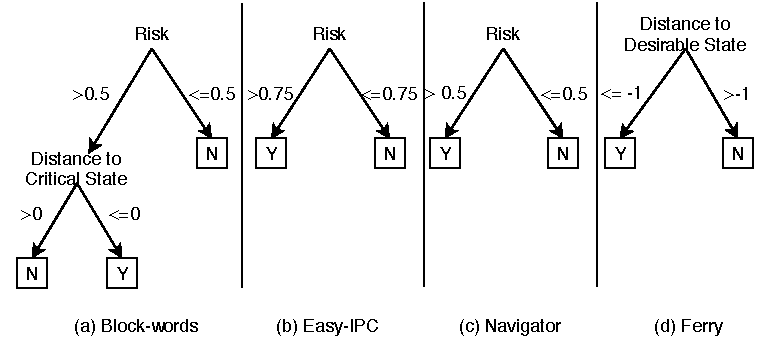
\includegraphics[width=2.5 in]{tree.pdf}}
			\label{fig:dt}
		\end{figure}
		%\item Use decision trees to derive a rule base to explain intervention
\begin{table}[]
\centering
\resizebox{\framewidth}{!}{%
\begin{tabular}{|l|l|l|l|}
\hline
\multicolumn{1}{|c|}{Domain} & \multicolumn{1}{c|}{Rules}                                 & \multicolumn{1}{c|}{Mapping}  & \multicolumn{1}{c|}{Effect}                                               \\ \hline
\multirow{4}{*}{BlocksWords} & Risk \textless{}= 0.5                                      & ``No risk of triggering undesirable state"   & N                                   \\ \cline{2-4} 
                             & Risk \textgreater 0.5                                      & ``Some risk of triggering undesirable state"   & -                                \\ \cline{2-4} 
                             & Dist. to Critical \textgreater 0 AND Risk \textgreater 0.5 & ``Somewhat high risk but undesirable state is not imminent" & N                   \\ \cline{2-4} 
                             & Dist. to Critical \textless{}= 0 AND Risk \textgreater 0.5 & ``Very high risk and undesirable state is imminent" & Y                           \\ \hline
\multirow{2}{*}{IPC-Grid+}   & Risk \textless{}=0.75                                      & ``No risk of triggering undesirable state"       & N                              \\ \cline{2-4} 
                             & Risk \textgreater 0.75                                     & ``Very high risk of triggering undesirable state"  & Y                            \\ \hline
\multirow{2}{*}{Navigator}   & Risk \textless{}= 0.5                                      & ``No risk of triggering undesirable state"        & N                             \\ \cline{2-4} 
                             & Risk \textgreater 0.5                                      & ``Very high risk of triggering undesirable state"   & Y                           \\ \hline
\multirow{2}{*}{Ferry}       & Dist. to desirable \textless{}= -1                         & ``Undesirable state is not imminent" & N \\ \cline{2-4} 
                             & Dist to desirable \textgreater -1                          & ``Undesirable state is imminent and occurs before reaching the desirable goal"           & Y                                 \\ \hline
\end{tabular}%
}
\end{table}
	\item $[$\texttt{Observation}$]$ $[$\texttt{Effect}$]$ because $[$\texttt{Mapping}$]$\\
{\small $[$\textsc{stack B A}$]$ $[$was interrupted$]$ because $[$very high risk and undesirable state is imminent$]$}
	\end{itemize}
\end{frame}

